%**************************************************************************
%* SpringSim 2019 Author Kit
%*
%* Word Processing System: TeXnicCenter and MiKTeX
%*
%**************************************************************************
\documentclass{scspaperproc}

\usepackage{latexsym}
\usepackage{graphicx}
\usepackage{mathptmx}

%
%****************************************************************************
% AUTHOR: You may want to use some of these packages. (Optional)
\usepackage{amsmath}
%\usepackage{amsfonts}
%\usepackage{amssymb}
%\usepackage{amsbsy}
%\usepackage{amsthm}
%****************************************************************************

%
%****************************************************************************
% AUTHOR: If you do not wish to use hyperlinks, then just comment
% out the hyperref usepackage commands below.

%% This version of the command is used if you use pdflatex. In this case you
%% cannot use ps or eps files for graphics, but pdf, jpeg, png etc are fine.

\usepackage[pdftex,colorlinks=true,urlcolor=blue,citecolor=black,anchorcolor=black,linkcolor=black]{hyperref}

%% The next versions of the hyperref command are used if you adopt the
%% outdated latex-dvips-ps2pdf route in generating your pdf file. In
%% this case you can use ps or eps files for graphics, but not pdf, jpeg, png etc.
%% However, the final pdf file should embed all fonts required which means that you have to use file
%% formats which can embed fonts. Please note that the final PDF file will not be generated on your computer!
%% If you are using WinEdt or PCTeX, then use the following. If you are using
%% Y&Y TeX then replace "dvips" with "dvipsone"

%% \usepackage[dvips,colorlinks=true,urlcolor=blue,citecolor=black,%
%% anchorcolor=black,linkcolor=black]{hyperref}

%% The use of the long citation format (e.g. "Brown and Edwards (1993)" rather than "[5]") and at the same
%% time using the hyperref package can lead to hard to trace bugs in case the citation is broken accross the
%% line (usually this will mark the entire paragraph as a hyperlink (clickable) which is easily noticeable and fixed
%% if using colorlinks, but not if the color is black -- as it is now). Worse yet, if a citation spans page boundary,
%% LaTeX compilation can fail, with an obscure error message. Since this depends a lot on the flow of the text
%% and wording, these bugs come and go and can be extremely hard for a beginner to trace. The error
%% message can look like this:
%%
%%    ! pdfTeX error (ext4): \pdfendlink ended up in different nesting level than \pdfstartlink.
%%    \AtBegShi@Output ...ipout \box \AtBeginShipoutBox 
%%    \fi \fi 
%%    l.174 
%%    ! ==> Fatal error occurred, no output PDF file produced!
%%
%% and can be universally fixed by putting an \mbox{} around the citation in question (in this case, at line 174)
%% and maybe adapting the wording a little bit to improve the paragraph typesetting, which is perhaps not
%% immediately obvious.
%****************************************************************************

%
%****************************************************************************
%*
%* AUTHOR: YOUR CALL!  Document-specific macros can come here.
%*
%****************************************************************************

\usepackage[]{algorithm2e}
\SetAlCapSty{} % caption of algorithms not bold
\usepackage{listings}

%#########################################################
%*
%*  The Document.
%*
\begin{document}

%***************************************************************************
% AUTHOR: AUTHOR NAMES GO HERE
% FORMAT AUTHORS NAMES Like: Author1, Author2 and Author3 (last names)
%
%		You need to change the author listing below!
%               Please list ALL authors using last name only, separate by a comma except
%               for the last author, separate with "and"
%
\SCSpagesetup{Thaler and Siebers}

% AUTHOR: Uncomment ONE of these correct conference names.
%\def\SCSconferenceacro{SpringSim}
\def\SCSconferenceacro{SummerSim}
%\def\SCSconferenceacro{AutumnSim}
%\def\SCSconferenceacro{PowerPlantSim}

% AUTHOR: Set the correct year of the conference.
\def\SCSpublicationyear{2019}

% AUTHOR: Set the correct month and dates; the dates are separated by a single minus sign
% with no spaces and no leading zeros, the month is a full name (e.g. April) with the first letter
% capitalized. For example, "April 8-13".
\def\SCSconferencedates{July 22-July 24}

% AUTHOR: Set the correct venue in the form "City, State, Country", for example "Los Angeles, CA, USA".
\def\SCSconferencevenue{Berlin, Germany}

% AUTHOR: Uncomment ONE of the track/symposium names where you are going to submit. Please, do NOT change.
% In case your symposium is not on this list, please DO contact your symposium chair.
%\def\SCSsymposiumacro{ANSS} % Annual Simulation Symposium
%\def\SCSsymposiumacro{CNS} % Communications and Networking Simulation Symposium
%\def\SCSsymposiumacro{HPC} % High Performance Computing Symposium
%\def\SCSsymposiumacro{TMS/DEVS} % Symposium on Theory of Modeling and Simulation
%\def\SCSsymposiumacro{ADS} % Agent-Directed Simulation
%\def\SCSsymposiumacro{MSCIAAS} % Modeling and Simulation of Complexity in Intelligent, Adaptive and Autonomous Systems
%\def\SCSsymposiumacro{MSM} % Modeling and Simulation in Medicine
%\def\SCSsymposiumacro{Mod4Sim} % Model-driven Approaches for Simulation Engineering Symposium
%\def\SCSsymposiumacro{Tutorial} % Tutorial Track
%\def\SCSsymposiumacro{WIP} % WIP Track
%\def\SCSsymposiumacro{Poster/Colloquium} % Poster Session and Student Colloquium
%\def\SCSsymposiumacro{MobileApp} % Student M\&S Mobile App Competition
%\def\SCSsymposiumacro{SPECTS} % Symposium on Performance Evaluation of Computer and Telecommunication Systems
\def\SCSsymposiumacro{SCSC} % Summer Computer Simulation Conference
%\def\SCSsymposiumacro{ICBGM} % International Conference on Bond-Graph Modeling
%\def\SCSsymposiumacro{Fossil} % Fossil Power Track
%\def\SCSsymposiumacro{Nuclear} % Nuclear Agent Power Track

% AUTHOR: Enter the title, all letters in upper case

%\newminted[HaskellCode]{haskell}{fontsize=\footnotesize}

% Title portion. Note the short title for running heads
\title{SHOW ME YOUR PROPERTIES! \\ The Potential Of Property-Based Testing In Agent-Based Simulation}
%\subtitle{The Potential Of Property-Based Testing In Agent-Based Simulation}

% AUTHOR: Enter the authors of the article, see end of the example document for further examples
\author{
\\%To level with the author block on the right.
Jonathan Thaler \\ 
Peer-Olaf Siebers \\ [12pt] 
School Of Computer Science \\
University of Nottingham \\
7301 Wollaton Rd \\
Nottingham, United Kingdom \\
\{jonathan.thaler,peer-olaf.siebers\}@nottingham.ac.uk\\
}

\maketitle

\section*{Abstract}
%OK	There should be no period at the end of the keywords list
%OK	The entire title needs to be 12pt all caps
%OK US English must be used. For example, "behaviour" should be "behavior"
%OK Footnotes are not allowed
%OK Five equations are given a single equation number, which does not match the required format for equations. They must either be listed within the text, or if listed separately than would each need to be on their own line with their own number.
%OK Code listing on page 4 should be in a listing environment instead of floating with no caption
%OK Need to ensure that all citations in text with at least 4 authors are written in abbreviated form
%OK Author biographies need to be added.

%OK On page 4 there is a reference to Listing 3, but I believe Listing 1 is meant.
%OK The hyperlinks in the text must show the URL such that someone reading a paper copy can see it. The recommended way (see the guidelines http://scs.org/authorskit) is to put the URL in the reference list, and add a citation in the text after the hyperlink.
%OK The De Vries reference in the reference list is incomplete and missing the period after the author name.
%OK The algorithm labels should not be bold, but regular text as with the rest of the caption.
%OK The listing caption should be underneath the listing.
%OK Using a citation as a noun should list the authors as part of the text, followed by the year. For example, “The paper (Onggo and Karatas 2016)...” should instead be written as “Onggo and Karatas (2016) say...”. There are a number of these situations within the paper that should be fixed.

This paper presents property-based testing, an approach for testing implementations of agent-based simulations (ABS), never considered so far in this field. It is a complementary technique to unit-testing and allows to test specifications and laws of an implementation directly in code which is then checked using \textit{automated} test-data generation. As case-studies, we present two different models, an agent-based SIR model and the SugarScape model, in which we will show how to apply property-based testing to explanatory and exploratory agent-based models and what its limits are.

\textbf{Keywords:} Agent-Based Simulation, Validation \& Verification, Property-Based Testing, Haskell

\maketitle

\section{Introduction}
There exists a large number of simulation packages which allow the convenient creation of System Dynamics simulations by straight-forward visual diagram creation. One simply creates stocks and flows, connects them, specifies the flow-rates and initial parameters and then runs the model. An example for such a visual diagram creation in the simulation package AnyLogic can be seen in Figure \ref{fig:sir_stockflow_diagram}.

\begin{figure}
	\centering
	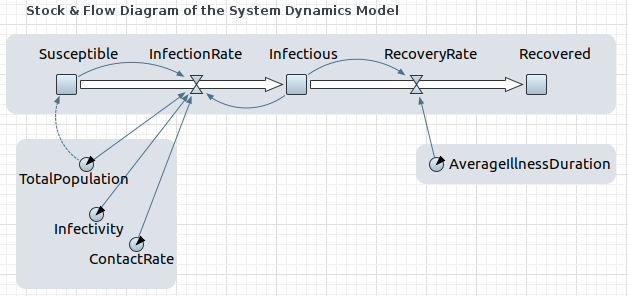
\includegraphics[width=.5\textwidth, angle=0]{./fig/SIR_SD_STOCKFLOW_DIAGRAMM.png}
	\caption{Visual System Dynamics Diagram of the SIR model in AnyLogic Personal Learning Edition 8.3.1.}
	\label{fig:sir_stockflow_diagram}
\end{figure}

Still, implementing System Dynamics directly in code is not as straight forward and involves numerical integration which can be quite tricky to get right. Thus, the aim of this paper is to look into how System Dynamics models can be implemented in code correctly without the use of a simulation package. We use the well known SIR model \cite{kermack_contribution_1927} from epidemiology to demonstrate our approach.

Our language of choice is Haskell because it emphasises a declarative programming style in which one describes \textit{what} instead of \textit{how} to compute. Further it allows to rule out interference with non-deterministic influences or side-effects already at compile-time. This is of fundamental importance for System Dynamics because it behaves completely deterministic and involves no stochastics or non-determinism whatsoever. Also, we make use of Functional Reactive Programming which allows to express continuous-time systems in a functional way. 

We show that by this approach we can arrive at correct-by-construction implementations of System Dynamic models. This means that the correctness of the code is obvious because we have closed the gap between the model specification and its implementation. Thus, the contribution of the paper is the demonstration of how to implement correct-by-construction System Dynamics simulations using Haskell and Functional Reactive Programming.

\section{Related Workd}
\label{sec:related}

% related works
% read all the papers peer has sent me
% https://www.atlassian.com/continuous-delivery/different-types-of-software-testing
%% TDD in ABS
Research on TDD of ABS is quite new and thus there exist relative few publications. The work \cite{collier_test-driven_2013} is the first to discusses how to apply the TDD approach to ABS, using unit-testing to verify the correctness of the implementation up to a certain level. They show how to implement unit-tests within the RePast Framework \cite{north_complex_2013} and make the important point that such a software need to be designed to be sufficiently modular otherwise testing becomes too cumbersome and involves too many parts. The paper \cite{asta_investigation_2014} discusses a similar approach to DES in the AnyLogic software toolkit. 

The paper \cite{onggo_test-driven_2016} proposes Test Driven Simulation Modelling (TDSM) which combines techniques from TDD to simulation modelling. The authors present a case study for maritime search-operations where they employ ABS. They emphasise that simulation modelling is an iterative process, where changes are made to existing parts, making a TDD approach to simulation modelling a good match. They present how to validate their model against analytical solutions from theory using unit-tests by running the whole simulation within a unit-test and then perform a statistical comparison against a formal specification. This approach will become of importance later on in our SIR case study.

The paper \cite{brambilla_property-driven_2012} propose property-driven design of robot swarms. They propose a top-down approach by specifying properties a swarm of robots should have from which a prescriptive model is created, which properties are verified using model checking. Then a simulation is implemented following this prescriptive and verified model after then the physical robots are implemented. The authors identify the main difficulty of implementing such a system that the engineer must \textit{"think at the collective-level, but develop at the individual-level}. It is arguably true that this also applies to implementing agent-based models and simulations where the same collective-individual separation exists from which emergent system behaviour of simulations emerges - this is the very foundation of the ABS methodology.

The paper \cite{gurcan_generic_2013} gives an in-depth and detailed overview over verification, validation and testing of agent-based models and simulations and proposes a generic framework for it. The authors present a generic UML class model for their framework which they then implement in the two ABS frameworks RePast and MASON. Both of them are implemented in Java and the authors provide a detailed description how their generic testing framework architecture works and how it utilises JUnit to run automated tests. To demonstrate their framework they provide also a case study of an agent-base simulation of synaptic connectivity where they provide an in-depth explanation of their levels of test together with code.

The review of the literature in the field gives the impression, that most research focuses on high-level validation and does not deal too much with verification on a technical, code-base level.

%% TDD in MAS
Although the work on TDD is scarce in ABS, there exists quite some research on applying TDD and unit-testing to multi-agent systems (MAS). Although MAS is a different discipline than ABS, the latter one has derived many technical concepts from the former one thus testing concepts applied to MAS might also be applicable to ABS. The paper \cite{nguyen_testing_2011} is a survey of testing in MAS. It distinguishes between unit tests which tests units that make up an agent, agent tests which test the combined functionality of units that make up an agent, integration tests which test the interaction of agents within an environment and observe emergent behaviour, system test which test the MAS as a system running at the target environment and acceptance test in which stakeholders verify that the software meets their goal. Although not all ABS simulations need acceptance and system tests, still this classification gives a good direction and can be directly transferred to ABS.  %Further the paper enumerates existing research and shows that some research is working on generating automated test input for agent level tests. 

%The paper \cite{tiryaki_sunit:_2007} discusses Test Driven Development in MAS and puts much emphasis on proposing agile processes to develop MAS software to handle complexity and continuously changing nature of requirements. The authors develop the SUNIT testing framework to implement unit-testing in an MAS environment.

\section{Property-Based Testing}
\label{sec:proptesting}

Property-based testing allows to formulate \textit{functional specifications} in code which then a property-based testing library tries to falsify by \textit{automatically} generating test-data, covering as many cases as possible. When a case is found for which the property fails, the library then reduces the test-data to its simplest form for which the test still fails e.g. shrinking a list to a smaller size. It is clear to see that this kind of testing is especially suited to ABS, because we can formulate specifications, meaning we describe \textit{what} to test instead of \textit{how} to test. Also the deductive nature of falsification in property-based testing suits very well the constructive and exploratory nature of ABS. Further, the automatic test-generation can make testing of large scenarios in ABS, which is almost always stochastic by nature, feasible as it does not require the programmer to specify all test-cases by hand, as is required in traditional unit-tests.

Property-based testing was invented by the authors of \cite{claessen_quickcheck_2000,claessen_testing_2002} in which they present the QuickCheck library in Haskell, which tries to falsify the specifications by \textit{randomly} sampling the space. We argue, that the stochastic sampling nature of this approach is particularly well suited to ABS, because it is itself almost always driven by stochastic events and randomness in the agents behaviour, thus this correlation should make it straight-forward to map ABS to property-testing. A challenge when using QuickCheck is to write \textit{custom} test-data generators for agents and the environment, which cover the space sufficiently enough to not miss out on important test-cases. According to the authors of QuickCheck \textit{"The major limitation is that there is no measurement of test coverage."} \cite{claessen_quickcheck_2000}. QuickCheck provides help to report the distribution of test-cases but still it could be the case that simple test-cases which would fail are never tested because of the stochastic nature of QuickCheck.

To give a rough idea on how property-based testing works in Haskell, we give a few examples of properties on lists, which are directly expressed as functions in Haskell. Such a function has to return a \textit{Bool}, which indicates \textit{True} in case the test succeeds or \textit{False} if not and can take input arguments which data is automatically generated by QuickCheck. Note that the first line of each function defines its name, its inputs (\textit{[Int]} is a list of integers) and the output which is the last type (\textit{Bool}). Note that the \textit{(++)} operator concatenates two lists, \textit{reverse} simply reverses a list.

\begin{HaskellCode}
-- concatenation operator (++) is associative
append_associative :: [Int] -> [Int] -> [Int] -> Bool
append_associative xs ys zs = (xs ++ ys) ++ zs == xs ++ (ys ++ zs)

-- reverse is distributive over concatenation (++)
-- xs and ys need to be swapped on the right-hand side!
reverse_distributive :: [Int] -> [Int] -> Bool
reverse_distributive xs ys = reverse (xs ++ ys) == reverse ys ++ reverse xs

-- the reverse of a reversed list is the original list
reverse_reverse :: [Int] -> Bool
reverse_reverse xs = reverse (reverse xs) == xs
\end{HaskellCode}

% POTENTIAL FOR SHORTENING
As a remedy for the potential sampling difficulties of QuickCheck, there exists also a deterministic property-testing library called SmallCheck \cite{runciman_smallcheck_2008}, which instead of randomly sampling the test-space, enumerates test-cases exhaustively up to some depth. It is based on two observations, derived from model-checking, that (1) \textit{"If a program fails to meet its specification in some cases, it almost always fails in some simple case"} and (2) \textit{"If a program does not fail in any simple case, it hardly ever fails in any case} \cite{runciman_smallcheck_2008}. This non-stochastic approach to property-based testing might be a complementary addition in some cases, where the tests are of non-stochastic nature with a search-space which is too large to implement manually by unit-tests but is relatively easy and small enough to enumerate exhaustively. The main difficulty and weakness of using SmallCheck is to reduce the dimensionality of the test-case depth search to prevent combinatorial explosion, which would lead to an exponential number of cases. Thus, one can see QuickCheck and SmallCheck as complementary instead of in opposition to each other.
% POTENTIAL FOR SHORTENING
Note that in this paper we only use QuickCheck due to the match of ABS stochastic nature and the random test generation. Also note that we regard property-based testing as \textit{complementary} to unit-tests and not in opposition - we see it as an addition in the TDD process of developing an ABS.

\section{Testing ABS implementations}
\label{sec:testingABS}

Generally we need to distinguish between two types of testing / verification in ABS.

\begin{enumerate}
	\item Testing / verification of models for which we have real-world data or an analytical solution which can act as a ground-truth - examples for such models are the SIR model, stock-market simulations, social simulations of all kind.
	\item Testing / verification of models which are of exploratory nature, inspired by real-world phenomena but for which no ground-truth per se exists - examples for such models is the Sugarscape \cite{epstein_growing_1996} or Agent\_Zero model \cite{epstein_agent_zero:_2014}.
\end{enumerate}

The baseline is that either one has an analytical model as the foundation of an agent-based model or one does not. In the former case, e.g. the SIR model, one can very easily validate the dynamics generated by the simulation to the one generated by the analytical solution through System Dynamics. In the latter case one has basically no idea or description of the emergent behaviour of the system prior to its execution e.g. SugarScape. In this case it is important to have some hypothesis about the emergent property / dynamics. The question is how verification / validation works in this setting as there is no formal description of the expected behaviour: we don't have a ground-truth against which we can compare our simulation dynamics.

One distinguishes between black-box and white-box verification where in white-box verification one looks directly at code and reasons about it whereas in black-box verification one generally feeds input to the software / functions / methods and compares it to expected output. Black-box verification is our primary concern in this paper as property-based testing is an instance of black-box verification. In the case of ABS we have the following levels of black-box tests:
\begin{enumerate}
	\item Isolated agent behaviour parts - test the individual parts which make up the agent behaviour under given inputs. For this we can use traditional unit-tests as shown by \cite{collier_test-driven_2013} and also property-based testing as we will show in the use-cases.
	\item Interacting agent behaviour - test if interaction between agents are correct. For this we can use traditional unit-tests as shown by \cite{collier_test-driven_2013}.
	\item Simulation dynamics - compare emergent dynamics of the ABS as a whole under given inputs to an analytical solution or real-world dynamics in case there exists some, using statistical tests. We see this type of tests conceptually as property-tests as well because we are testing properties of the model / simulation as we will see in the use-cases. Technically speaking we can both use traditional unit-tests and also property-based tests to implement them - conceptually they are property-tests.
	\item Hypotheses - test whether hypotheses about the model are valid or invalid. This is very similar to the previous point but without comparing it to analytical solutions or real-world dynamics but only to some hypothetical values.
\end{enumerate}

\section{Case Study I: SIR}
\label{sec:case_SIR}

As first use-case we discuss property-based testing for the agent-based SIR model. It is a very well studied and understood compartment model from epidemiology \cite{kermack_contribution_1927} which allows to simulate the dynamics of an infectious disease like influenza, tuberculosis, chicken pox, rubella and measles spreading through a population. We implemented an agent-based version of this model \footnote{The code is freely accessible from \url{https://github.com/thalerjonathan/phd/tree/master/public/propabs/sir}}, which is inspired by \cite{macal_agent-based_2010}.

In this model, people in a population of size $N$ can be in either one of three states \textit{Susceptible}, \textit{Infected} or \textit{Recovered} at a particular time, where it is assumed that initially there is at least one infected person in the population. People interact \textit{on average} with a given rate of $\beta$ other people per time-unit and become infected with a given probability $\gamma$ when interacting with an infected person. When infected, a person recovers \textit{on average} after $\delta$ time-units and is then immune to further infections. An interaction between infected persons does not lead to re-infection, thus these interactions are ignored in this model. Due to the models origins in System Dynamics (SD) \cite{porter_industrial_1962}, there exists a top-down formalisation in SD with the following equations:

\begin{equation}
\frac{\mathrm d S}{\mathrm d t} = -infectionRate \\ 
\frac{\mathrm d I}{\mathrm d t} = infectionRate - recoveryRate \\ 
\frac{\mathrm d R}{\mathrm d t} = recoveryRate 
\end{equation}

\begin{equation}
infectionRate = \frac{I \beta S \gamma}{N} \\
recoveryRate = \frac{I}{\delta} 
\end{equation}

\subsection{Deriving a property}
Our goal is to derive a property which connects the agent-based implementation to the SD equations. The foundation are both the infection- and recovery-rate where the infection-rate determines how many \textit{Susceptible} agents per time-unit become \textit{Infected} and the recovery-rate determines how many \textit{Infected} agents per time-unit become \textit{Recovered}. Lets look at the pseudo-code of the susceptible agent behaviour, which is key for the infection-rate:

\begin{algorithm}
generate on average $\beta$ make-contact events per time-unit\; 
\If{make-contact event}{
  select random agent \textit{randA} from population\; 
  \If{agent randA infected}{
    become infected with probability $\gamma$\; 
  }  
}
\caption{Susceptible behaviour}
\end{algorithm}

Per time-unit, a susceptible agent makes \textit{on average} contact with $\beta$ other agents where in the case of a contact with an infected agent the susceptible agent becomes infected with a given probability $\gamma$. In this description there is another probability hidden, which is the probability of making contact with an infected agent which is simply the ratio of number of infected agents to number non-infected agents. We can now derive the formula for the probability of a \textit{Susceptible} agent to become infected: $\beta * \gamma * \frac{number of infected}{number of non-infected}$. When we look at the formula we can see that it is conceptually the same representation of the \textit{infection-rate} of the SD specification as shown above - except that it only considers a single \textit{Susceptible} agent instead of the aggregate of \textit{S} susceptible agents. We have now a property we can check using a property-based test.

\subsection{Constructing the property-based test}
Having a property (law), we want now to construct a property-based test for it. The formula is invariant under random population mixes and thus should hold for varying agent populations where the mix of \textit{Susceptible, Infected and Recovered} agents is random - thus we use QuickCheck to generate the population randomly, the property must still hold.

Obviously we need to pay attention to the fact that we are dealing with a stochastic system thus we can only talk about averages and thus it does not suffice to only run a single agent but we are repeating this for e.g. 10.000 \textit{Susceptible} agents (all with different random-number seeds). 

To check whether this test has passed we compare the required amount of agents which on average should become infected using the above formula to the one from our tests (simply count the agents which got infected and divide by N) and if the value lies within some small $\epsilon$ then we accept the test as passed. Now we can construct the following property-based test as shown in Algorithm \ref{alg:prop_test_infectionrate}.

\begin{algorithm}
\SetKwInOut{Input}{input}\SetKwInOut{Output}{output}
\Input{List \textit{randAs} of random agent-population generated by QuickCheck}
populationCount     = length \textit{randAs}\;
infectedCount       = count \textit{Infected} in \textit{randAs}\;
infectionRate       = infectivity * contactRate * (infectedCount / populationCount)\;

susceptibles = 10000\;
countInfected = 0\;
\For{$i\leftarrow 1$ \KwTo $susceptibles$}{
  create \textit{Susceptible} agent sa\;
  run agent sa for 1.0 time-unit, with list \textit{randAs} as input\;
  \If{agent sa became \textit{Infected} }{
	countInfected = countInfected + 1\;
  }
}

actualInfectionRate = countInfected / susceptibles\;
$\epsilon$ = 0.1\;
\eIf{abs (actualInfectionRate - infectionRate) $\leq \epsilon$}{
  PASS\;
} {
  FAIL\;
}
\caption{Property-based test for infection-rate.}
\end{algorithm}
\label{alg:prop_test_infectionrate}

When running, QuickCheck generates 100 random test-cases by randomly generating 100 different \textit{randAs} inputs to the test. All have to pass for the whole property-test to pass, which should be the case with an $\epsilon = 0.1$. 

This is the very power which property-based testing is offering us: we directly express the specification of the original SD model in a test of our agent-based implementation and let QuickCheck generate random test cases for us. This closely ties our implementation to the original specification and "proves" that it is actually a valid implementation.

%\subsection{Infected Behaviour}
%An infected agent will \textit{always} recover after some finite time, which is \textit{on average} after $\delta$ time-units. Note that this property involves stochastics too, so to test this property we run a large number of infected agents e.g. $N = 10.000$ (all with different random-number seeds) until they recover, record the time of each agents recovery and then average over all recovery times. To check whether this test has passed we compare the average recovery times to $\delta$ and if they lie within some small $\epsilon$ then we accept the test as passed (note again that we could use a t-test for better stochastic robustness but this is not the point of this paper).
%
%TODO: clearly state the property we test
%
%TODO: produce some pseudo-code of how the property-test conceptually works
%
%in the infected agent test we check if the average duration is as specified. does this resemble the recovery rate? or in other words: can we somehow test the recovery rate?
%durationsAvg = sum durations / fromIntegral (length durations)
%
%We use property-testing with QuickCheck in this case as well to generate the set of other agents as input for the infected agents. Strictly speaking this would not be necessary as an infected agent never makes contact with other agents and simply ignores them - we could as well just feed in an empty list. We opted for using QuickCheck for the following reasons:
%
%\begin{itemize}
%	\item We wanted to stick to the interface specification of the agent-implementation as close as possible which asks to pass the states of all agents as input.
%	\item We shouldn't make any assumptions about the actual implementation and if it REALLY ignores the other agents, so we strictly stick to the interface which requires us to input the states of all the other agents.
%	\item The set of other agents is ignored when determining whether the test has failed or not which indicates by construction that the behaviour of an infected agent does not depend on other agents.
%	\item We are not just running a single replication over 10.000 agents but 100 of them which should give black-box verification more strength.
%\end{itemize}
%
%\subsection{Recovered Behaviour}
%A recovered agent will stay recovered \textit{forever}. Obviously we cannot write a property-based test that truly verifies that because it had to run in fact \textit{forever}. In this case we need to resort to white-box verification and look directly at the code and reason whether this property holds true.

\section{Case Study II: SugarScape}
\label{sec:case_sug}
We now look at how property-based testing can be made of use in the \textit{exploratory} Sugarscape model \cite{epstein_growing_1996}. It was one of the first models in ABS, with the aim to \textit{grow} an artificial society by simulation and connect observations in their simulation to phenomenon observed in real-world societies. In this model a population of agents move around in a discrete 2D environment, where sugar grows, and interact with each other and the environment in many different ways. The main features of this model are (amongst others): searching, harvesting and consuming of resources, wealth and age distributions, population dynamics under sexual reproduction, cultural processes and transmission, combat and assimilation, bilateral decentralized trading (bartering) between agents with endogenous demand and supply, disease processes transmission and immunology. For our research we undertook a \textit{full and validated} implementation of the Sugarscape model \footnote{The code can be accessed freely from \url{https://github.com/thalerjonathan/haskell-sugarscape}}. We validated of our implementation against the book \cite{epstein_growing_1996} and a NetLogo implementation \cite{weaver_replicating_2009} \footnote{\url{https://www2.le.ac.uk/departments/interdisciplinary-science/research/replicating-sugarscape}} during which we also implemented property tests. Due to lack of space we added a discussion of the validation process as an Appendix \ref{app:validation}.

Whereas in the explanatory SIR case-study we had an analytical solution, inspired by the SD origins of the model, the fundamental difference in the exploratory Sugarscape model is that no such analytical solutions exist. This raises the question, which properties we can actually test in such a model - we propose the following:

\begin{itemize}
	\item Environment behaviour - the Sugarscape environment has its own behaviour which boils down to regrowing of resources. The correct working can be tested using property-tests by generating random environments and checking laws governing the regrowth.
	
	\item Agent behaviour - obviously full agent behaviour could be tested with property-tests, using randomly generated agents (with random values in their properties). It turned out to be quite difficult to derive properties for full agent behaviour, thus in this paper we restricted ourselves to test parts of agent behaviour and also left out testing of agent interactions.

	\item Emergent behaviour - although we don't have analytical descriptions of properties of our model in the case of Sugarscape, there still exist informal descriptions and more formal hypotheses about emergent properties. Property-testing can be used to check them and if proved to be valid can be seen as regression tests.
\end{itemize}

\subsection{Environment behaviour}
The environment in the Sugarscape model has some very simple behaviour: each site has a sugar level and when harvested by an agent, it regrows back to the full level over time. Depending on the configuration of the model it either grows back immediately within 1 tick or over multiple ticks. We can construct simple property-tests for these behaviours. In the case the sugar grows back immediately, we let QuickCheck generate a random environment and then run the environment behaviour for 1 tick and then check the property that all sites have to be back to their maximum sugar level. In the case of regrow over multiple ticks, we also use QuickCheck to generate a random environment but additionally a random \textit{positive} rate (which is a floating point number) which we then use to calculate the number of ticks until full regrowth. After running the random environment for the given number of ticks all sites have to be back to full sugar level - see Algorithm \ref{alg:prop_test_rateregwroth} for this case.

Note that QuickCheck initially doesn't know how to generate a random environment because each site consists of a custom data-structure for which QuickCheck is not able to generate random instances by default. This problem is solved by writing a custom data-generator, for which existing QuickCheck functions can be used e.g. picking the current sugar level of a site from a random range.

\begin{algorithm}
\SetKwInOut{Input}{input}\SetKwInOut{Output}{output}
\Input{Random environment \textit{env} generated by QuickCheck}
\Input{Random regrowth rate \textit{randRate} generated by QuickCheck}
maxTicks = maxSugarCapacityOnSites / randRate\;
env' = runEnvironmentTicks maxTicks env\;
sites = getEnvironmentSites env'\;

\eIf{all sites maxSugarLevel}{
  PASS\;
} {
  FAIL\;
}
\caption{Property-based test for rate-based regrow of sugar on all sites.}
\label{alg:prop_test_rateregwroth}
\end{algorithm}

The Sugarscape environment is a torus where the coordinates wrap around in both dimensions. To check whether the implementation of the wrapping calculation is correct we used both unit- and property-tests. With the unit-tests we carefully constructed all possible cases we could think of and came up with 13 test-cases. With the property-based test we simply defined a single test-case where we expressed the property, that after wrapping \textit{any} random coordinates supplied by QuickCheck, the wrapped coordinates have to be within bounds. See Algorithm \ref{alg:prop_test_wrapcoords}.

\begin{algorithm}
\SetKwInOut{Input}{input}\SetKwInOut{Output}{output}
\Input{Random 2D discrete coordinate \textit{randCoord} generated by QuickCheck}
(x, y) = wrapCoordinates randCoord\;

\eIf{(x $\geq$ 0 and x $\leq$ environmentDimX) and (y $\geq$ 0 and y $\leq$ environmentDimY)}{
  PASS\;
} {
  FAIL\;
}
\caption{Property-based test for wrap-coordinates functionality.}
\label{alg:prop_test_wrapcoords}
\end{algorithm}

\subsection{Agent behaviour}
We implemented a number of property-tests for agent functions which just cover a part of an agents behaviour: checks whether an agent has died of age or starved to death, the metabolism, immunisation step, check if an agent is a potential borrower or fertile, lookout, trading transactions. We provided custom data-generators for the agents and let QuickCheck generate the random data and us running the agent with the provided data, checking for the properties. 

As an example, provided in Algorithm \ref{alg:prop_test_agent}, we give the property-test of an agent dying of age, which happens when the agents age is greater or equal its maximum age. It might look trivial but property-based testing helps us here to clearly state the invariants (properties) and relieves us from constructing all possible edge-cases because we rely on QuickChecks abilities to cover them for us.

\begin{algorithm}
\SetKwInOut{Input}{input}\SetKwInOut{Output}{output}
\Input{Random agent \textit{ag} with random age generated by QuickCheck}
died = hasAgentDiedOfAge ag;\

\eIf{died == (age ag >= maxAge ag)} {
  PASS\;
} {
  FAIL\;
}
\caption{Property-based test for agent dying of age.}
\label{alg:prop_test_agent}
\end{algorithm}

\subsection{Emergent properties}
In the validation and verification process of our Sugarscape implementation we put informal descriptions and hypotheses about emergent properties from the Sugarscape book into formal property-tests. Examples for such hypotheses / informal descriptions of emergent properties are e.g. the carrying capacity becomes stable after 100 steps; when agents trade with each other, after 1,000 steps the standard deviation of trading prices is less than 0.05; when there are cultures, after 2,700 steps either one culture dominates the other or both are equally present.

The property we test for is whether \textit{the emergent property under test is stable under varying random-number seeds} or not. Put another way, we let QuickCheck generate random number streams and require that the tests all pass. Unfortunately, this revealed that this property doesn't hold for all hypotheses. The problem is that QuickCheck generates by default 100 test-cases for each property-test where all need to pass for the whole property-test to pass - this wasn't the case, where most of the 100 test-cases passed but unfortunately not all. Thus in this case a different approach is required: instead of requiring \textit{every} test to pass we require that \textit{most} tests pass, which can be achieved using a T-test with a confidence interval of e.g. 95\%. This means we won't use QuickCheck anymore and resort to a normal unit-test where we run the simulation 100 times with different random number streams each time and then performing a T-test with a 95\% confidence interval. Note that we are now technically speaking of a unit-test but conceptually it is still a property-test.

In Algorithm \ref{alg:prop_test_trading} we show a property-test for checking whether after 1,000 steps the standard deviation of trading prices is less than 0.05. The test passes if out of 100 runs a 95\% confidence interval is reached using a T-test.

\begin{algorithm}
maxTicks = 1000\;
replications = 100\;
stdAverage = 0.05\;
tradingPriceStdsList = empty list\;

\For{$i\leftarrow 1$ \KwTo replications}{
rng = new random number generator\;
simContext = initSimulation rng\;
out = runSimulation maxTicks simContext\;
tps = extractTradingPrices out\;
tpsStd = calculate standard deviation of tps\;
insert tpsStd into tradingPriceStdsList\;
}

tTestPass = perform 1-sided t-test comparing stdAverage with tradingPriceStdsList on a 0.95 interval\;

\eIf{tTestPass}{
  PASS\;
} {
  FAIL\;
}
\caption{Property-based test for trading prices.}
\label{alg:prop_test_trading}
\end{algorithm}

\chapter{Conclusions}
\label{chap:concl}

\section{Being Realistic}
It is of most importance to stress that we don't condemn the current state-of-the-art approach of object-oriented specification and implementation to ABS. The strength of object-oriented programming is surely that it can be seen as \textit{programming as modelling} and thus will be always an attractive approach to ABS. Also we are realists and know that there are more points to consider when selecting a set of methods for developing software for an ABS than robustness, verification and validation. Almost always the popularity of an existing language and which languages the implementer knows is the driving force behind which methods and languages to choose. This means that ABS will continue to be implemented in object-oriented programming languages and many perfectly well functioning models will be created by it in the future. Although they all suffer from the same issues mentioned in the introduction this doesn't matter as they are not of central importance to most of them.
Nonetheless we think our work is still essential and necessary as it may start a slow paradigm-shift and opens up the minds of the ABS community to a more functional and formal way of approaching and implementing agent-based models and simulations and recognizing the benefits one gets automatically from it by doing so.

\section{What we are not doing}
Because of this highly interdisciplinary topic we explicitly mention what we do not want to undertake in this PhD.
First we don't want to develop another language for formal agent-specification which needs to be compiled or used in some fancy tool - we want to put it directly into Haskell, building on the existing facilities.
Second, we are not developing a new economic theory about decentralized bilateral bartering, we take the existing theory and existing agent-based models and apply our methods to them.
Third, we don't want to use fancy statistics and number juggling for comparing validating and verifying models: we want structural comparison (category-theory).
Fourth, we do NOT want to do a direct comparison of object-orientation vs. functional in ABS, as we would get lost in an infinite amount of low-level technical details. We look at the benefits / drawbacks more on a conceptual level, applied to ABS.

\section*{Acknowledgments}
The authors would like to thank J. Hey for valuable feedback and discussions.

% Please don't change the bibliographystyle style
\bibliographystyle{scsproc}
% AUTHOR: Include your bib file here
\bibliography{propabs.bib}

\section*{Author Biographies}
\textbf{\uppercase{JONATHAN THALER}} is a Ph.D. student at the University of Nottingham and part of the Intelligent Modelling and Analysis Group (\url{http://www.cs.nott.ac.uk/~psxjat/}). His main research interest is the benefits and drawbacks of using pure functional programming with Haskell for implementing Agent-Based Simulations.

\textbf{\uppercase{Dr. PEER-OLAF SIEBERS}} is an Assistant Professor at the School of Computer Science, University of Nottingham, UK (\url{http://www.cs.nott.ac.uk/~pszps/}). His main research interest is the application of computer simulation to study human-centric complex adaptive systems. He is a strong advocate of Object Oriented Agent-Based Social Simulation. This is a novel and highly interdisciplinary research field, involving disciplines like Social Science, Economics, Psychology, Operations Research, Geography, and Computer Science. His current research focuses on Urban Sustainability and he is a co-investigator in several related projects and a member of the university's "Sustainable and Resilient Cities" Research Priority Area management team.

\end{document}